\documentclass{standalone}
\usepackage{graphicx}	
\usepackage{amssymb, amsmath}
\usepackage{color}

\usepackage{tikz}
\usetikzlibrary{arrows.meta, math}
\usepackage{pgfmath}

\definecolor{light}{RGB}{220, 188, 188}
\definecolor{mid}{RGB}{185, 124, 124}
\definecolor{dark}{RGB}{143, 39, 39}
\definecolor{highlight}{RGB}{180, 31, 180}
\definecolor{gray10}{gray}{0.1}
\definecolor{gray20}{gray}{0.2}
\definecolor{gray30}{gray}{0.3}
\definecolor{gray40}{gray}{0.4}
\definecolor{gray60}{gray}{0.6}
\definecolor{gray70}{gray}{0.7}
\definecolor{gray80}{gray}{0.8}
\definecolor{gray90}{gray}{0.9}
\definecolor{gray95}{gray}{0.95}

\newcommand{\fiber}[2]{
  \pgfmathsetmacro{\x}{#1}
  \draw [color=#2, line width=1]
      (\x, -2) .. controls (\x - 0.75, -1) and (\x + 0.5, -0.25) 
   .. (\x + 0.5, 0.25) .. controls (\x + 0.5, 0.75) and (\x - 0.5, 1.25) .. (\x + 0.25, 2)
}

\begin{document}

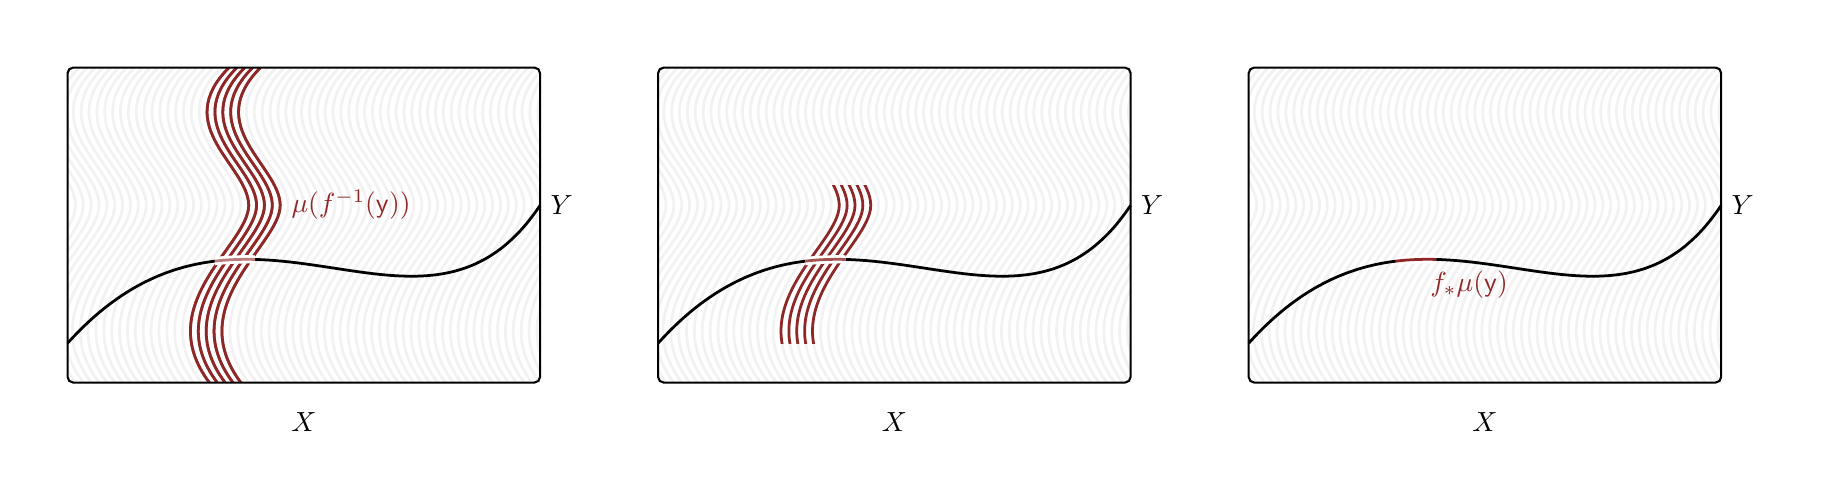
\begin{tikzpicture}[scale=1]

  \begin{scope}[shift={(0, 0)}] 
    \draw[white] (-3.5, -3) rectangle (4, 2.5);
     
    % Input Space
    \begin{scope}
      \clip (-3, -2) rectangle (3, 2);
      
      \foreach \x in {-3.4, -3.3, ..., 3.5} {
        \fiber{\x}{gray95};    
      }  
    \end{scope}
         
    \begin{scope}
      \clip (-3, -2) rectangle (3, 2);
      
      \foreach \x in {-1.2, -1.1, ..., -0.8} {
        \fiber{\x}{mid};    
      }  
    \end{scope}
    
    \begin{scope}
      \clip (-3, -2) rectangle (3, 2);
      
      \foreach \x in {-1.2, -1.1, ..., -0.8} {
        \fiber{\x}{dark};    
      }  
    \end{scope}
    
    \node[dark] at (0.6, 0.26) { $\mu(f^{-1}( \mathsf{y} ))$ };
    
    \draw [rounded corners=2, color=black, line width=0.75] (-3, -2) rectangle (3, 2);
    \node at (0, -2.5) { $X$ };  
    
    % Output Space
    \draw [line width=1] (-3, -1.5) .. controls (-0.75, 1) and (1.5, -2) .. (3, 0.25)
    node[right] { $Y$ };
    
    \begin{scope}
      \clip (-1.13, -2) rectangle (-0.62, 2);
      \draw [white, line width=3] (-3, -1.5) .. controls (-0.75, 1) and (1.5, -2) .. (3, 0.25);
      \draw [mid, line width=1] (-3, -1.5) .. controls (-0.75, 1) and (1.5, -2) .. (3, 0.25);
    \end{scope}
  \end{scope}
  
  \begin{scope}[shift={(7.5, 0)}] 
    \draw[white] (-3.5, -3) rectangle (4, 2.5);
     
    % Input Space
    \begin{scope}
      \clip (-3, -2) rectangle (3, 2);
      
      \foreach \x in {-3.4, -3.3, ..., 3.5} {
        \fiber{\x}{gray95};    
      }  
    \end{scope}
         
    \begin{scope}
      \clip (-3, -2) rectangle (3, 2);
      
      %\foreach \x in {-1.2, -1.1, ..., -0.8} {
      %  \fiber{\x}{mid};    
      %}  
    \end{scope}
    
    \begin{scope}
      \clip (-3, 0.5) rectangle (3, -1.5);
      
      \foreach \x in {-1.2, -1.1, ..., -0.8} {
        \fiber{\x}{dark};    
      }  
    \end{scope}
    
    \draw [rounded corners=2, color=black, line width=0.75] (-3, -2) rectangle (3, 2);
    \node at (0, -2.5) { $X$ };  
    
    % Output Space
    \draw [line width=1] (-3, -1.5) .. controls (-0.75, 1) and (1.5, -2) .. (3, 0.25)
    node[right] { $Y$ };
    
    \begin{scope}
      \clip (-1.13, -2) rectangle (-0.62, 2);
      \draw [white, line width=3] (-3, -1.5) .. controls (-0.75, 1) and (1.5, -2) .. (3, 0.25);
      \draw [mid!50!dark, line width=1] (-3, -1.5) .. controls (-0.75, 1) and (1.5, -2) .. (3, 0.25);
    \end{scope}
  \end{scope}
  
  \begin{scope}[shift={(15, 0)}] 
    \draw[white] (-3.5, -3) rectangle (4, 2.5);
     
    % Input Space
    \begin{scope}
      \clip (-3, -2) rectangle (3, 2);
      \foreach \x in {-3.4, -3.3, ..., 3.5} {
        \fiber{\x}{gray95};    
      }  
    \end{scope}
         
    \begin{scope}
      %\clip (-3, -2) rectangle (3, 2);
      %\foreach \x in {-1.2, -1.1, ..., -0.8} {
      %  \fiber{\x}{mid};    
      %}  
    \end{scope}
    
    \draw [rounded corners=2, color=black, line width=0.75] (-3, -2) rectangle (3, 2);
    \node at (0, -2.5) { $X$ };  
    
    % Output Space
    \draw [line width=1] (-3, -1.5) .. controls (-0.75, 1) and (1.5, -2) .. (3, 0.25)
    node[right] { $Y$ };
    
    \begin{scope}
      \clip (-1.13, -2) rectangle (-0.62, 2);
      \draw [white, line width=3] (-3, -1.5) .. controls (-0.75, 1) and (1.5, -2) .. (3, 0.25);
      \draw [dark, line width=1] (-3, -1.5) .. controls (-0.75, 1) and (1.5, -2) .. (3, 0.25);
    \end{scope}
    
    \node[dark] at (-0.2, -0.75) { $f_{*} \mu(\mathsf{y})$ };
  \end{scope}
\end{tikzpicture}

\end{document}  